\chapter{Statistical Analysis}
To estimate the sensibility of the $tH$ signal, we define an Asimov dataset, made by replacing the ensemble of simulated backgrounds and signal by a single one. The statistical uncertainty of the Asimov data is calculated as $\sqrt{n}$, with $n$ the number of events. The uncertainty of the signal strength is estimated by applying a  fit to the Asimov dataset, where the model
is constructed from the sum of the individual backgrounds and signal. The fit is implemented using a Poisson likelihood and gaussian constraints for the systematical uncertainties in the model.


\section{Likelihood and fit procedure}
The likelihood function is the product of Poisson probabilities for all bins of the BDT distribution. The likelihood function has the form
\begin{align}
L(\mu,\alpha)=\prod_{j=1}^{N}\frac{(\mu s_j +b_j)^{n_j}}{n_j !}e^{-(\mu s_j+b_j)} \prod_{k=1}^M e^{\frac{-\alpha^2_k}{2}}
\end{align}
where $N$ is the total number of bins, $n_j$ is the number of events in a bin $j$,  $s_j$ is the number of signal events, µ is a parameter that modifies the signal strength and  $b_j$ is the number of background events.
$b_j$ is the sum of different background processes $k$
\begin{align}
b_j=\sum_k b_j^k(1+ \alpha_k \sigma_k)
\end{align}
$\alpha_k$ is the parameter that modifies the expected background prediction and $\sigma_k$ is the systematic uncertainty of the associated background. \\

The fit is applied by minimizing the $-\log{L}$ (NLL) with respect to the parameter $\mu$ and $\alpha_k$. The minimization is performed by using the package ROOFIT \cite{roofit}.
%log es usado para evitar valores extremadamente pequenos debido a los productos de los exponenciales
%negativo es para hacer una minimizacion, positivo es maximizacion


\begin{table}[ht!]
	\centering
	\caption{Postfit  yields for the fit to the Asimov data corresponding to 35.9 /fb. The uncertainty given is the combined statistical plus systematic.}
\begin{tabular}{ccc}
	\hline
	Process  & SM    & $k_t=-1$ \\
	\hline
$t\bar{t}W$  &  68$\pm$8.9& 68 $\pm$8.9 \\
	$t\bar{t}Z$  & 25.9$\pm$3.8&25.9$\pm$3.8\\
$WZ$ &  15.1$\pm$7.4& 15.1$\pm$7.4\\
Rares &  20.8$\pm$4.8& 20.8$\pm$4.8 \\
	Fakes  &  80.9$\pm$9.0&  80.9$\pm$8.9 \\
	$t\bar{t}H$  &   24.2$\pm$2.0 &  24.2$\pm$2.0 \\
\hline
$tH$&  2.1$\pm$16.5 &26.2$\pm$13.1 
\end{tabular}
\label{table1}
\end{table}

In the figure \ref{simple} and table \ref{table1} , shows the results of the model fitting using the Asimov data for both models. As mentioned before, the  $k_t=-1$, the number of events for the $tH$ signal is more than ten times, compared to SM. This improves the sensitivity to the signal. Due to the small number of signal events the uncertainty for the SM is large compared to the $k_t$=-1 scenario, where the uncertainty is around 50$\%$. In this analysis only the signal is affected by the change $k_t$=1 (SM) $\rightarrow$  $k_t=-1$, therefore the backgrounds remain the same.
\begin{figure}[!htbp]
	\centering
	\begin{minipage}[b]{0.48\textwidth}
		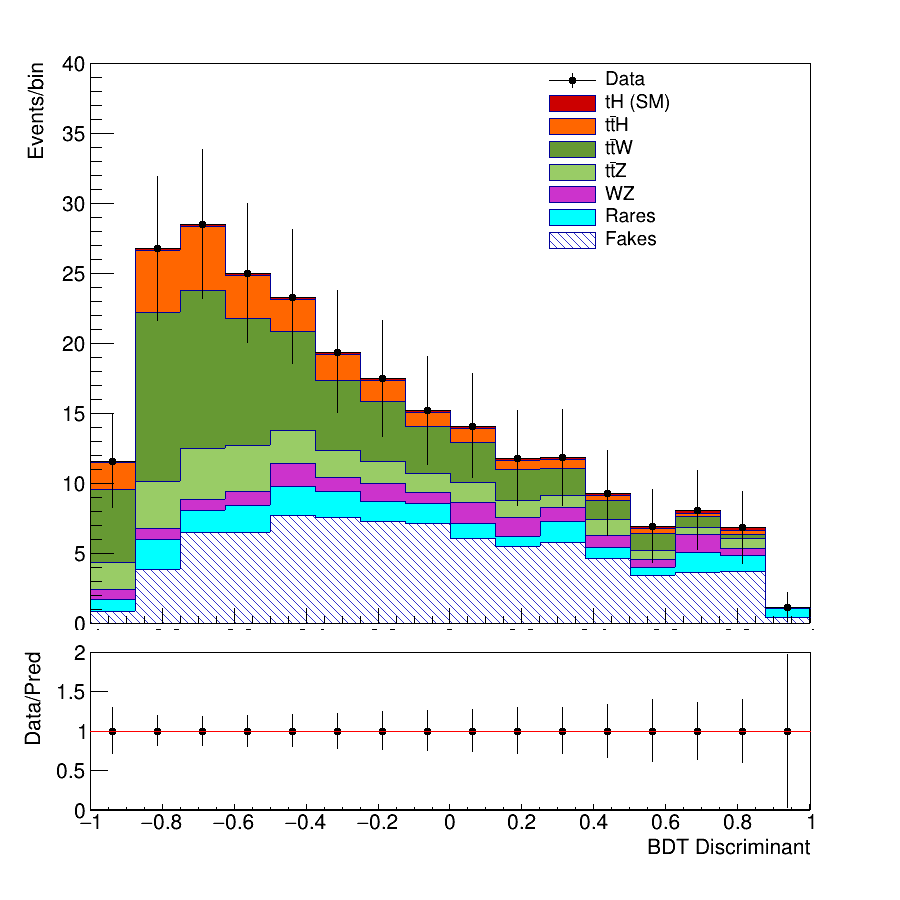
\includegraphics[width=\textwidth]{Chapter4/simple.png}
	\end{minipage}
	\hfill
	\begin{minipage}[b]{0.48\textwidth}
		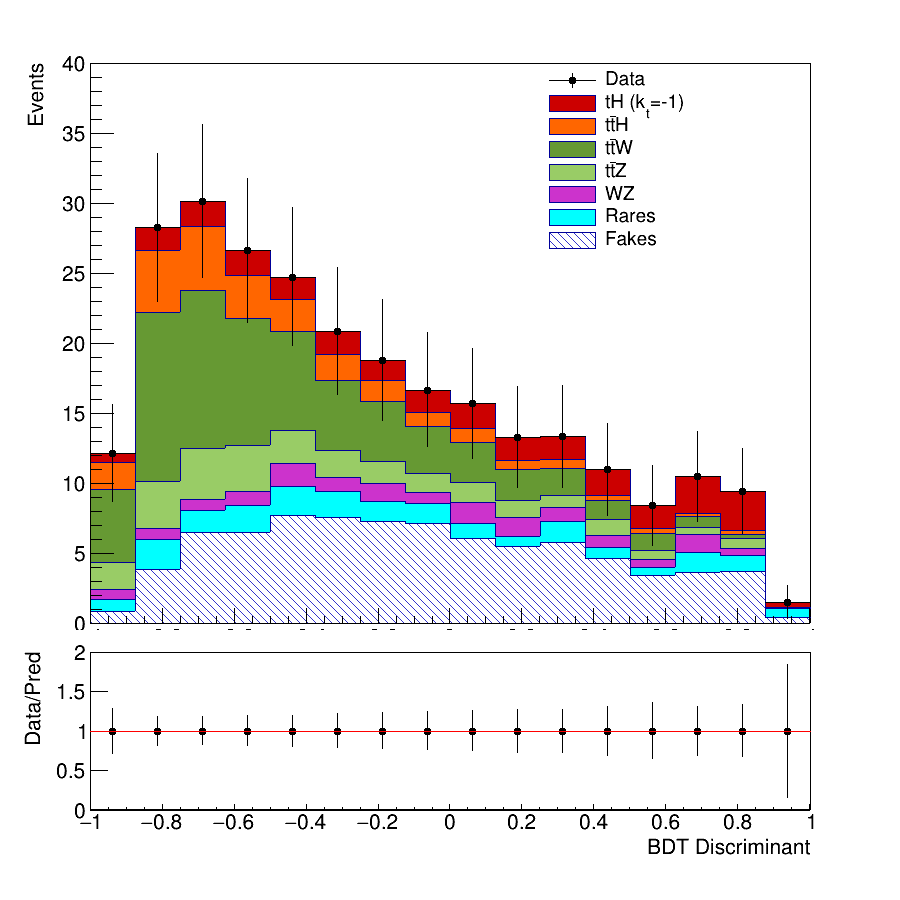
\includegraphics[width=\textwidth]{Chapter4/simple-kt-1.png}
	\end{minipage}
	\caption{Post fit signal and background yields for tH process for SM (Left) and $k_t=-1$ (Right).
		In the box below each distribution, the ratio of the observed and predicted event yields is shown}
\label{simple}
\end{figure}
In the table \ref{parameters}, shows the $\mu$ and $\alpha$ parameters. For the pre-fit, values of $\alpha$ are set to zero and $\mu$ is set to 1.After the fit,  $\alpha$ parameters set to zero indicates that in the fit, the values of the backgrounds didn't changed for the SM and the $\mu$ parameter set to 1 indicates that the signal strength also didn't changed.
\begin{table}[ht]
	\centering
	\caption{$\alpha$ and $\mu$ values  for the fit to Asimov data corresponding to 35.9 fb$^{-1}$}
	\begin{tabular}{ccc}
		\hline
		Parameter  & SM &kt\\
		$\mu$   & 1.00 $\pm$  7.74& 1.0 $\pm$  0.5\\
		$\alpha_{t\bar{t}W}$&  0.00 $\pm$  0.89&  0.00 $\pm$  089\\
		$\alpha_{t\bar{t}Z}$ &  0.00 $\pm$  0.98& 0.00 $\pm$  0.98\\
		$\alpha_{WZ}$   & 0.00 $\pm$  0.97& 0.00 $\pm$  0.97\\
		$\alpha_{Rares}$   &0.00 $\pm$  0.95&0.00 $\pm$  0.98 \\
		$\alpha_{Fakes}$ &   0.00 $\pm$  0.96& 0.00 $\pm$  0.95\\
		$\alpha_{t\bar{t}H}$ &0.00 $\pm$  0.98& 0.00 $\pm$ 0.98\\
	\end{tabular}
\label{parameters}
\end{table}


\section{Limit calculation}
Due to the large background, the signal strength for the Asimov data with 35.9 $fb^{-1}$ is consistent with zero.
Therefore, we estimate an upper limit on the signal strength at 95$\%$  confidence level.\\

We can define the likelihood ratio
\begin{align}
\lambda(\mu,\alpha)=\frac{L(\mu,\alpha)}{L(\hat{\mu},\hat{\alpha})}
\end{align}
Where $\hat{\alpha}$ and $\hat{\mu}$ are the parameters obtained in the previous section which correspond to the minimal of the NLL.
To determine an upper limit on the strength parameter $\mu$ , we use the following statistical test
\begin{align}
q=  -2\ln{\lambda(\mu)} 
\end{align}
High values of $q$ represent greater incompatibility between the data and the fit model.
$q$ is a random variable with a $\chi^2$ distribution \cite{asimov}.


\begin{figure}[ht!]
	\centering
	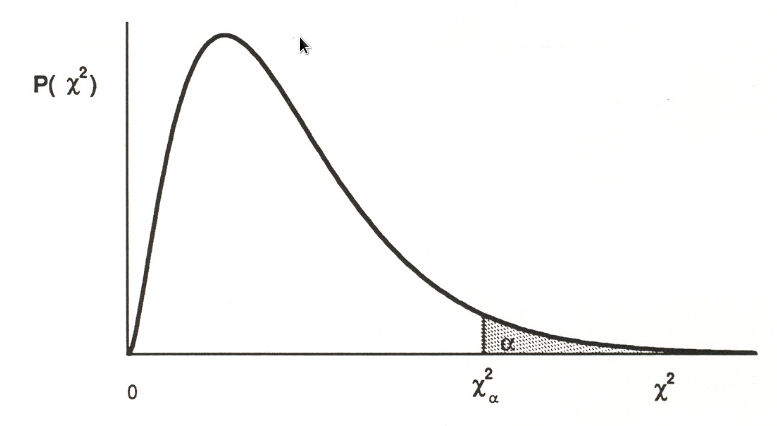
\includegraphics[scale=0.5]{Chapter4/chi_squared.png}
	\caption{Illustration of the $\chi^2$ distribution used for the limit estimation}
\label{chi}
\end{figure}
 
In order to find the upper limit value of $\mu$, we search for the largest value of $\mu$  such that $q$ remains below the shaded region shown in \ref{chi}, where $\alpha$=0.05 in this case. 
It is useful to scan $q$ as function of $\mu$ , which is normally a parabolic function as shown in \ref{scanl}.In the SM case, the scan has a wider shape in comparison to the $k_t$=-1. This is due to larger statistical uncertainty on the $\mu$ parameter. \\

Using the above technique, we find an expected upper limit $\mu < $17.008 for SM model and $\mu < $ 2.378 for $k_t$=-1 model.


\begin{figure}[!htbp]
	\centering
	\begin{minipage}[b]{0.48\textwidth}
		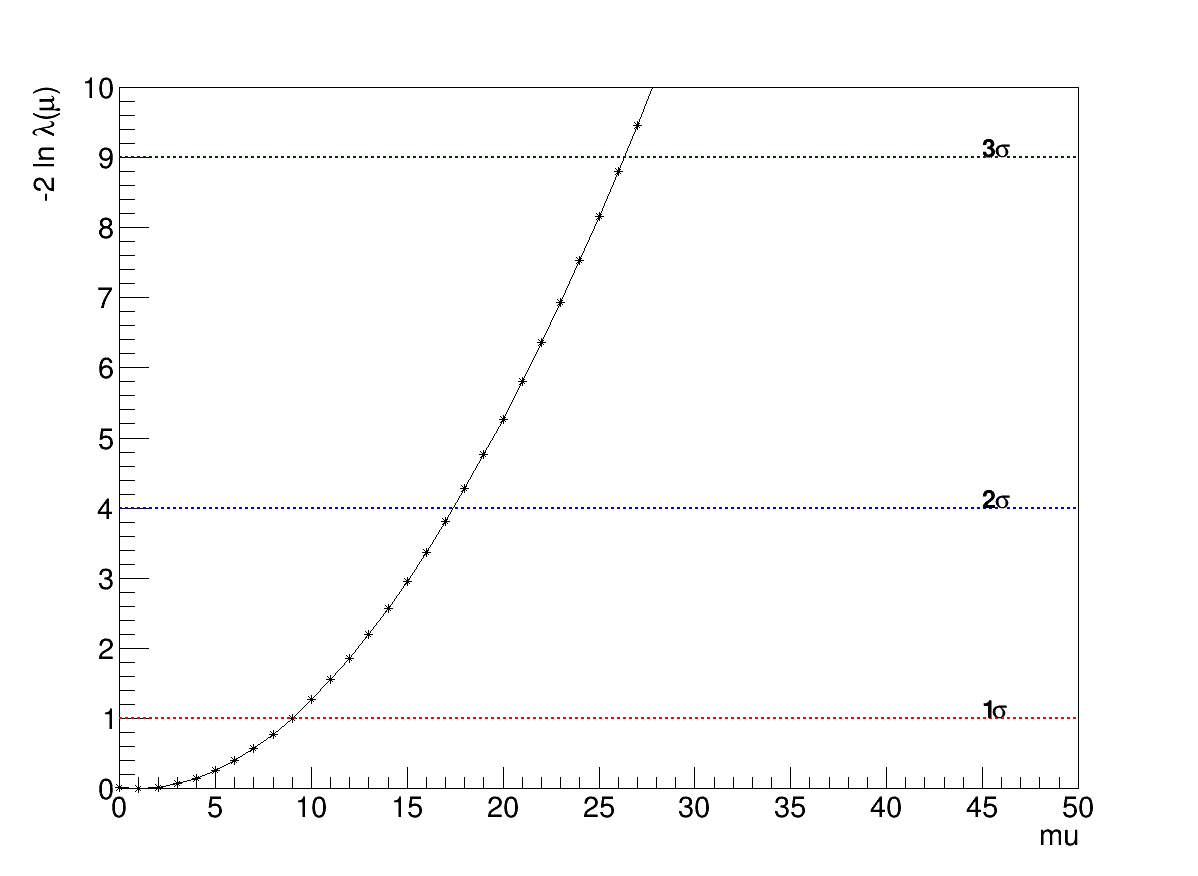
\includegraphics[width=\textwidth]{Chapter4/Likelihood.png}
	\end{minipage}
	\hfill
	\begin{minipage}[b]{0.48\textwidth}
		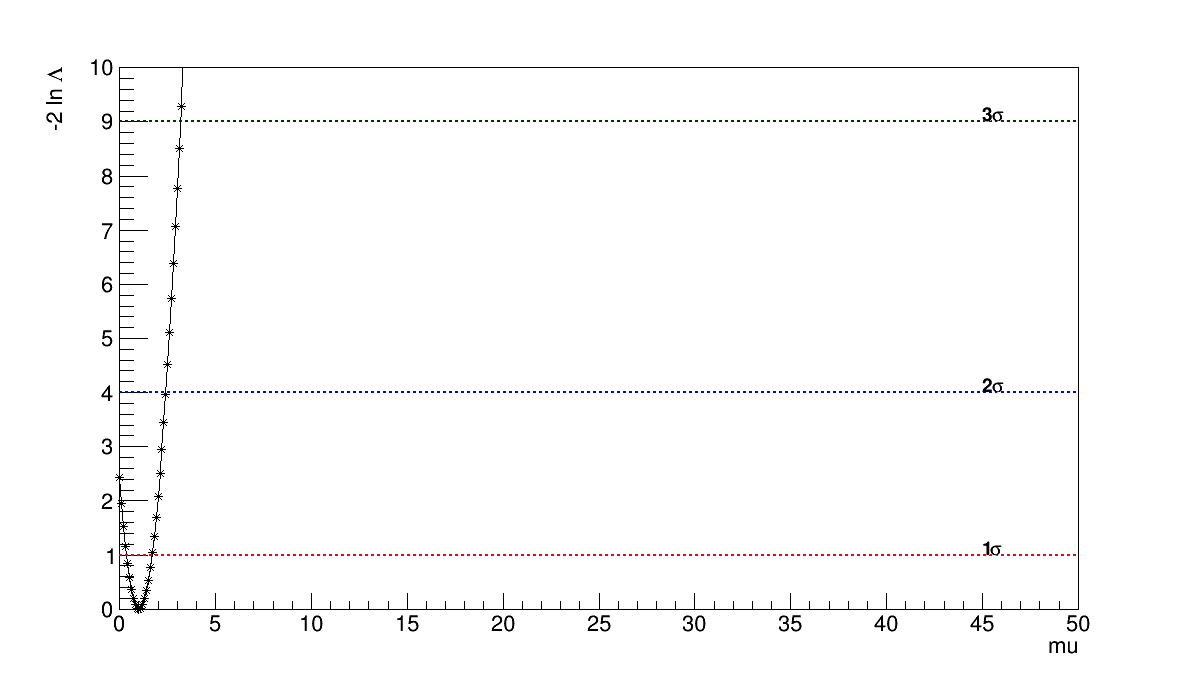
\includegraphics[width=\textwidth]{Chapter4/Likelihood-kt-1.png}
	\end{minipage}
	\caption{Likelihood scan for SM (Left) and $k_t$=-1 (Right)}
	\label{scanl}
\end{figure}


\section{Extrapolation for higher luminosities}


\begin{table}[ht!]
	\caption{Estimation of $\mu$ and upper limits for Asimov extrapolations}
	\begin{tabular}{|c|c|c|c|c|}
		\hline
		Luminosity (fb$^{-1}$)	&$\mu$ &$\mu$ for $k_t=-1$ &$\mu$ upper limit &$\mu$ upper limit for $k_t=-1$ \\
		\hline
		35.9 & 1.00 $\pm$  8.32 & 1.00 $\pm$  0.249&	22.328 & 2.777   \\
		\hline
		150& 1.00 $\pm$  6.44 & 1.00 $\pm$  0.544  &12.619 &0.915 \\
		\hline
		300&1.00 $\pm$  4.83 &1.00 $\pm$  0.407 & 9.427&0.649 \\
		\hline
		3000&1.00 $\pm$  1.54 & 1.00 $\pm$  0.151&	 3.442 & 0.25
		\\
		\hline
	\end{tabular}
\end{table}


